% Snowflake Data Engineering — Chapter 4 | original manuscript draft
% Author: Arman Golbidi | Editorial snapshot: 21 October 2026
% Compile: xelatex -interaction=nonstopmode -halt-on-error Snowflake_Data_Engineering_Chapter_03.tex
% Trim: 178 x 254 mm; margins inside 23 mm / outside 17 mm / top-bottom 19 mm.
% Body: 10.75 pt / 13.65 pt leading = 1.27 line-height ratio; code: 8.75 pt.
\documentclass[11pt,twoside]{article}
\usepackage[paperwidth=178mm,paperheight=254mm,inner=23mm,outer=17mm,top=19mm,bottom=19mm,headheight=5mm,headsep=4mm,footskip=9mm]{geometry}
\usepackage{fontspec}
\setmainfont{LibertinusSerif-Regular.otf}[BoldFont=LibertinusSerif-Bold.otf,ItalicFont=LibertinusSerif-Italic.otf,BoldItalicFont=LibertinusSerif-BoldItalic.otf]
\setsansfont{LibertinusSans-Regular.otf}[BoldFont=LibertinusSans-Bold.otf,ItalicFont=LibertinusSans-Italic.otf]
\setmonofont{LibertinusMono-Regular.otf}[Scale=0.91]
\usepackage[english]{babel}
\usepackage{microtype}
\usepackage{setspace}
\setstretch{1.0}
\usepackage{titlesec,enumitem,tabularx,array,booktabs,needspace,fancyhdr,lastpage}
\usepackage[most]{tcolorbox}
\usepackage{tikz}
\usetikzlibrary{arrows.meta,positioning,fit,shapes.misc,calc}
\usepackage{listings}
\usepackage{xcolor}
\usepackage{hyperref}
\usepackage{amsmath}
\hypersetup{colorlinks=true,urlcolor=steelblue,linkcolor=steelblue,pdfauthor={Arman Golbidi},pdftitle={Snowflake Data Engineering - Chapter 4: Snowflake SQL and Data Modeling},pdfsubject={English technical book manuscript, fourth chapter, 178 x 254 mm}}
\definecolor{navy}{HTML}{15334A}
\definecolor{steelblue}{HTML}{17779B}
\definecolor{teal}{HTML}{12888A}
\definecolor{lightblue}{HTML}{ECF5F7}
\definecolor{papergray}{HTML}{F2F5F6}
\definecolor{inkgray}{HTML}{4A5862}
\definecolor{thinrule}{HTML}{CBD7DB}
\AtBeginDocument{\color{navy}\fontsize{10.75}{13.65}\selectfont}
\setlength{\parindent}{0pt}
\emergencystretch=1.3em
\setlength{\parskip}{3.3pt plus 0.7pt minus 0.6pt}
\setlist[itemize]{leftmargin=4mm,itemsep=1pt,topsep=2pt,parsep=0pt}
\setlist[enumerate]{leftmargin=5mm,itemsep=1pt,topsep=2pt}
\titleformat{\section}{\sffamily\bfseries\color{navy}\fontsize{14}{17}\selectfont}{}{0pt}{}
\titlespacing*{\section}{0pt}{8pt}{4pt}
\titleformat{\subsection}{\sffamily\bfseries\color{steelblue}\fontsize{10.8}{13}\selectfont}{}{0pt}{}
\titlespacing*{\subsection}{0pt}{5pt}{1pt}
\newcommand{\topic}[2]{\subsection*{#1\quad #2}}
\newcommand{\repo}[2]{\par\begingroup\fontsize{8.0}{9.6}\selectfont\sffamily\color{inkgray}\textbf{Project reference:} \href{#2}{#1}. \textit{Not independently executed; rights review pending.}\par\endgroup}
\newtcolorbox{insight}[1][]{enhanced,breakable,colback=lightblue,colframe=thinrule,boxrule=.45pt,arc=1.3mm,left=2.8mm,right=2.8mm,top=1.8mm,bottom=1.8mm,before skip=5pt,after skip=5pt,#1}
\newtcolorbox{whitebox}[1][]{enhanced,breakable,colback=papergray,colframe=thinrule,boxrule=.35pt,arc=1mm,left=2.6mm,right=2.6mm,top=1.5mm,bottom=1.5mm,before skip=4pt,after skip=5pt,#1}
\lstdefinestyle{chaptercode}{basicstyle=\ttfamily\fontsize{8.75}{10.7}\selectfont,backgroundcolor=\color{papergray},frame=single,framerule=.35pt,rulecolor=\color{thinrule},breaklines=true,columns=fullflexible,keepspaces=true,showstringspaces=false,aboveskip=5pt,belowskip=5pt,xleftmargin=2mm,xrightmargin=1mm,framexleftmargin=2mm,framexrightmargin=1mm}
\lstset{style=chaptercode}
\pagestyle{fancy}
\fancyhf{}
\fancyhead[LE]{\sffamily\fontsize{7.6}{9}\selectfont\color{inkgray}\textsc{Snowflake Data Engineering}}
\fancyhead[RO]{\sffamily\fontsize{7.6}{9}\selectfont\color{inkgray}\textsc{04 / SQL and Data Modeling}}
\fancyfoot[LE,RO]{\sffamily\bfseries\fontsize{8.2}{9}\selectfont\color{steelblue}\thepage}
\fancyfoot[LO,RE]{\sffamily\fontsize{7.6}{9}\selectfont\color{inkgray}Arman Golbidi \quad | \quad Chapter 04}
\renewcommand{\headrulewidth}{0.35pt}
\renewcommand{\footrulewidth}{0pt}
\setcounter{page}{57}
\raggedbottom

% CHAPTER 04 ONLY, pages 57--76 in the planned book
\begin{document}
% page 57
{\sffamily\bfseries\color{teal}\fontsize{10}{12}\selectfont CHAPTER 04\quad /\quad SQL \& DATA MODELLING}\par\vspace{2mm}
{\sffamily\bfseries\color{navy}\fontsize{23}{26}\selectfont Snowflake SQL and\par Data Modeling}\par
\vspace{1.6mm}{\color{steelblue}\rule{\linewidth}{1.5pt}}\par\vspace{2mm}
{\sffamily\color{inkgray}\fontsize{11.1}{14.5}\selectfont The query can be correct and the dashboard can still be wrong.}\par\vspace{2mm}

At 07:30 a Finnish energy analyst notices that yesterday's generation total increased after a supplier corrected an earlier file. A straightforward \texttt{SUM} now reports a larger value, although the physical electricity production has not changed. In the raw observations, both the original and the corrected measurement remain. The database has faithfully retained both versions; the analytical model has accidentally counted both.

This chapter moves from knowing where Snowflake stores and executes data to understanding \emph{what a row means}. Correct SQL is more than grammatical SQL. It is a precise contract between business events, timestamps, units, identifiers, and consumers. We will first learn expression semantics, then build relational transformations, and finally establish an auditable dimensional model for the Finland Energy Analytics platform introduced in Chapter 1.

\begin{insight}\textbf{Our engineering decision}\par
What is the unique observation we promise to deliver, and which SQL transformations and independent tests prove that the resulting energy number is neither duplicated nor silently discarded?\end{insight}

\textbf{By the end of the chapter, you should be able to:}
\begin{itemize}
\item choose appropriate Snowflake numeric, string and temporal data types;
\item predict join multiplicity, null handling, and aggregation results;
\item use common table expressions, windows, and \texttt{QUALIFY} defensibly;
\item distinguish UTC observations from Finland's local reporting calendar;
\item specify a fact-table grain, dimensions, surrogate keys, and history rules;
\item build SQL data-quality checks and reconcile source and target totals; and
\item document, review, and test an energy-model implementation.
\end{itemize}
\textbf{Prerequisites.} Chapters 2--3, a non-production Snowflake schema, and basic \texttt{SELECT}. The accompanying CSV validator runs offline; Snowflake-specific SQL is prepared for a reviewable live test and is \emph{not} presented as already executed.

\begin{whitebox}\textbf{Reading path.}\quad Sections 4.1--4.4 establish query semantics; 4.5--4.7 define durable data objects and grain; 4.8--4.9 develop evidence and maintainability. The guided laboratory creates the first analytical gold-layer model.\end{whitebox}

\newpage
% page 58
\section*{4.1\quad Snowflake SQL syntax and data types}
\topic{4.1.1}{Primitive types and temporal types}
A column type is an assertion about meaning. \texttt{VARCHAR} can preserve an incoming reading exactly, but does not establish that it is a usable quantity. A \texttt{NUMBER(18,3)} expresses a fixed decimal scale; a \texttt{FLOAT} describes approximate numerical representation and should not be chosen for monetary reconciliations or comparisons that require exact decimal equality. Measurement systems may still use floating-point computations, but the trade-off must be explicit.

Snowflake's \texttt{NUMBER(p,s)} has configurable precision and scale. Choose the scale from the resolution of the source measurement rather than from the number of decimal places that happen to appear in one demonstration file. For our energy case, \texttt{NUMBER(18,3)} is an illustrative representation of MWh reported to three decimals; it is not a universal rule for energy markets. The distinction between MWh (energy over an interval) and MW (power at an instant or averaged over an interval) will become important when defining the fact.

\begin{center}
\small\begin{tabularx}{\linewidth}{@{}p{31mm}X@{}}\toprule
Type family & Typical modelling decision\\\midrule
\texttt{VARCHAR} & Raw identifiers, source text, source-system codes; define normalization rules.\\
\texttt{NUMBER(p,s)} & Exact fixed-scale measures and surrogate integer identifiers.\\
\texttt{FLOAT} & Approximate calculations when their numerical limitations are acceptable.\\
\texttt{BOOLEAN} & Validated flags; distinguish false from missing.\\
\texttt{DATE} & Civil/calendar day with no instant or timezone.\\
\texttt{TIMESTAMP\_NTZ} & Wall-clock value with no timezone semantics encoded; document convention.\\
\texttt{TIMESTAMP\_LTZ} & Instant displayed relative to the session timezone.\\
\texttt{TIMESTAMP\_TZ} & Instant with stored numeric offset, not a permanent zone name.\\\bottomrule
\end{tabularx}
\end{center}

\begin{lstlisting}[language=SQL,caption={Type choices; intended for a dedicated book schema.}]
CREATE TABLE energy_reading_example (
    source_code       VARCHAR(32) NOT NULL,
    interval_start_utc TIMESTAMP_NTZ NOT NULL,
    energy_mwh        NUMBER(18,3),
    is_estimated      BOOLEAN
);
\end{lstlisting}
\textbf{Decision test.} If a source provides \texttt{2026-10-25 02:30} without offset or timezone, no temporal type can tell you which occurrence of that local clock reading it meant. Preserve raw evidence and demand a timezone contract before treating the value as an instant. Official type and conversion definitions should be checked against Snowflake's SQL reference [1, 2].

\newpage
% page 59
\topic{4.1.2}{Snowflake SQL dialect distinctions}
A useful working assumption is that Snowflake uses familiar relational SQL plus dialect-specific constructs. The danger is not obvious syntax differences; it is code that appears portable but changes meaning. \texttt{QUALIFY}, for instance, filters after window expressions have been evaluated. \texttt{LIMIT} controls a returned row count but does not imply a repeatable row sample without \texttt{ORDER BY}. An identifier can also be case-sensitive when double-quoted, whereas unquoted identifiers are normally normalized by Snowflake. Build a stable naming policy instead of depending on implicit rules.

A \emph{session} supplies defaults such as role, warehouse, database, schema, and timezone. The same SQL text can therefore behave differently in separate sessions when it relies on implicit context. For reproducible examples, set or check the context first. A teaching query should favor explicit column names and an explicit order when result order matters.

\begin{lstlisting}[language=SQL,caption={Inspect session context before reproducing a lesson.}]
SELECT CURRENT_ROLE()       AS active_role,
       CURRENT_DATABASE()   AS active_database,
       CURRENT_SCHEMA()     AS active_schema,
       CURRENT_WAREHOUSE()  AS active_warehouse,
       CURRENT_SESSION()    AS session_id;

-- Inspect the current timezone setting separately:
SHOW PARAMETERS LIKE 'TIMEZONE' IN SESSION;
\end{lstlisting}

Three SQL statements should be distinguished: \texttt{CREATE TABLE} defines a durable contract; \texttt{CREATE VIEW} defines a query-backed interface; and \texttt{CREATE TABLE AS SELECT} materializes a query result at a particular moment. They are not interchangeable simply because each can produce a tabular result. Similarly, \texttt{WHERE} applies row-level filtering before aggregation; \texttt{HAVING} filters grouped output; \texttt{QUALIFY} filters results of window functions. Confusing their logical positions creates subtle errors.

\begin{whitebox}\textbf{Maintainability rule.}\quad Every published listing identifies its expected database/schema, assumed permissions and whether it mutates data. A command taken out of a chapter should not accidentally target a reader's production dataset.\end{whitebox}

Snowflake lets analysts express much of the platform's logic declaratively. That is a strength when the data model and tests are clear: transformations become inspectable, reviewable artifacts. It is a liability when a team treats a successful run as proof of business correctness. Later sections will formalize a model test that is independent of the transformation under test.
\repo{P035: SQL and Python analytics guide}{https://github.com/Snowflake-Labs/sfguide-getting-started-with-data-analytics-with-sql-python}


\textbf{A reproducibility check.} When copying SQL from another database, review every cast, timestamp literal, identifier and null predicate rather than assuming the two dialects are equivalent. A good migration test runs the same small input through both implementations and compares data types, row grain and null values as well as displayed results. This catches cases where a query returns the expected number of rows but subtly changes their meaning.

\newpage
% page 60
\topic{4.1.3}{CAST, TRY\_CAST, and NULL behavior}
Data enters analytics in forms chosen by the source, not by the warehouse. A reading may arrive as \texttt{'12.500'}, \texttt{'N/A'}, the empty string, or a JSON null. \texttt{CAST} (and the shorthand \texttt{::}) expresses a conversion that fails when an incompatible value is encountered. \texttt{TRY\_CAST} returns SQL \texttt{NULL} rather than an error for supported conversions of \emph{string} expressions. For other inputs, use an appropriate \texttt{TRY\_TO\_*} conversion function. Silent conversion failure is an exception that must be counted, not a data-cleaning strategy [2].

\begin{lstlisting}[language=SQL,caption={Do not equate an invalid value with zero.}]
WITH incoming(raw_mwh) AS (
  SELECT column1 FROM VALUES
    ('12.500'), ('N/A'), (''), (NULL)
)
SELECT raw_mwh,
       TRY_TO_DECIMAL(raw_mwh, 18, 3) AS parsed_mwh,
       IFF(raw_mwh IS NOT NULL AND
           TRY_TO_DECIMAL(raw_mwh,18,3) IS NULL,
           'REJECT', 'REVIEW') AS parse_status
FROM incoming;
\end{lstlisting}

SQL has three-valued logic. A predicate comparing a number to \texttt{NULL} is neither true nor false; it evaluates to unknown. \texttt{WHERE} retains rows for which its predicate is true. Thus \texttt{energy\_mwh <> 0} excludes rows with null energy as well as zeros. To test missingness, use \texttt{IS NULL}; to supply a fallback, use \texttt{COALESCE} only when that fallback has an explicit business meaning. Replacing an unknown electricity reading with zero can manufacture an apparent outage.

\begin{insight}\textbf{Failure path: a quiet conversion error}\par
A source sends \texttt{'1,25'} in a locale that uses the comma as decimal separator. A generic numeric conversion may return null or fail, depending on its expression and format. The engineering response is to specify the source contract, normalize deliberately, retain the original value, and measure rejection counts---not to silently drop the row.\end{insight}

\textbf{Verification check.} Given an input list containing a valid decimal, a textual flag, an empty string and a missing field, predict the \texttt{TRY\_TO\_DECIMAL} results before executing the query. Explain why the proportion of rejected rows should be monitored separately from the aggregate produced from valid rows.


\textbf{What to do with failed parses.} Keep a rejection table containing the raw value, source row, reason code, ingestion batch and original timestamp string. Report a rejection rate as rejected source events divided by evaluated events, and distinguish completely missing fields from invalid, present text. A corrected record should be able to enter the accepted dataset without erasing the rejected input, so that investigations can reconstruct what the system actually received.

\newpage
% page 61
\section*{4.2\quad Filtering, joins, aggregations, and subqueries}
\topic{4.2.1}{SELECT, JOIN, and filters}
For the remainder of the chapter, suppose the engineering team has a record for each source's delivered hourly energy: source, metric, start timestamp, MWh, ingestion timestamp, and source-row identity. The \emph{source-row identity} is an audit key; it is not automatically the key of the business observation. A correction may arrive with a different row identity but refer to the same source, metric and hour.

Start with a query that narrows both columns and time range. A bounded UTC interval is easier to reason about than local-date text when clocks change. Half-open intervals, \texttt{>= start} and \texttt{< end}, also compose without boundary double-counting.
\begin{lstlisting}[language=SQL,caption={Bounded fact query: no implicit all-time scan.}]
SELECT source_code, interval_start_utc, energy_mwh
FROM book_ch04.fact_energy_hourly
WHERE interval_start_utc >=
      '2026-01-15 00:00:00'::TIMESTAMP_NTZ
  AND interval_start_utc <
      '2026-01-16 00:00:00'::TIMESTAMP_NTZ;
\end{lstlisting}

\topic{4.2.2}{GROUP BY, HAVING, and subqueries}
\texttt{GROUP BY} changes the grain of a query. Every grouping key is part of the output grain, and aggregated measures describe that set of rows. \texttt{HAVING} applies conditions after grouping. A subquery can express a reusable threshold or compare a group to a scalar derived from another relation. Before optimizing a query, write its intended \emph{result key} in plain language.
\begin{lstlisting}[language=SQL,caption={Daily energy by source, after quality filtering.}]
SELECT source_code,
       TO_DATE(interval_start_utc) AS utc_day,
       SUM(energy_mwh) AS total_mwh
FROM book_ch04.fact_energy_hourly
GROUP BY source_code, utc_day
HAVING SUM(energy_mwh) > 0
ORDER BY utc_day, source_code;
\end{lstlisting}

\textbf{Boundary.} This query is correct only if the fact already contains one accepted value for each promised observation. Aggregating raw retries first and deduplicating later cannot generally recover the true total. That is why the key is part of query design rather than an optional performance optimization.
\repo{P036: dbt TPC-H relational example}{https://github.com/clausherther/dbt-tpch}


\textbf{Worked question.} Suppose two independent sites produce 10 and 20 MWh during the same UTC hour. Grouping by hour alone yields 30 MWh; grouping by site and hour yields two separate values. Both queries are mathematically consistent, but they answer different business questions. Before choosing the aggregation keys, decide whether sites can represent overlapping boundaries or duplicated market reporting; if so, summation across sites requires additional business logic.

\newpage
% page 62
\topic{4.2.3}{Duplicate rows and incorrect join cardinality}
A join combines rows based on a predicate. It does \emph{not} guarantee one result per row from the left relation. If one energy source joins to two history records in a dimension, one fact row becomes two result rows; \texttt{SUM} then double-counts its energy even if every input was individually valid. This is called a \emph{fanout}. It is among the most expensive semantic mistakes in analytics because it produces believable numbers.

\begin{center}
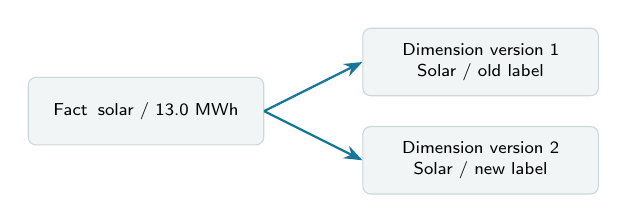
\begin{tikzpicture}[scale=.78,transform shape,>=Stealth, every node/.style={font=\sffamily\fontsize{8.2}{10}\selectfont},bx/.style={draw=thinrule,rounded corners=1mm,fill=papergray,align=center,minimum height=11mm,text width=36mm}]
\node[bx] (f) {Fact\: solar / 13.0 MWh};
\node[bx,right=16mm of f,yshift=8mm] (d1) {Dimension version 1\\ Solar / old label};
\node[bx,right=16mm of f,yshift=-8mm] (d2) {Dimension version 2\\ Solar / new label};
\draw[->,thick,steelblue] (f.east) -- (d1.west);
\draw[->,thick,steelblue] (f.east) -- (d2.west);
\end{tikzpicture}
\end{center}
\textit{Figure 4.1.} A join on \texttt{source\_code} alone duplicates a fact when a dimension has multiple historical versions.

Check cardinality \emph{before} relying on the join. A source dimension for type-2 history needs an effective-date join, or a fact that already stores the appropriate version's surrogate key. A type-1 dimension should have a unique natural key. Use two independent tests: one for dimension-key uniqueness and one for result-count preservation when a one-to-one relationship is expected.

\begin{lstlisting}[language=SQL,caption={Detect a dimension key that is not unique.}]
SELECT source_code, COUNT(*) AS versions
FROM book_ch04.dim_source
GROUP BY source_code
HAVING COUNT(*) > 1;
-- Only valid as a defect test for Type 1 dimensions.
\end{lstlisting}

A join to a dimension can also \emph{lose} facts when written as an inner join and a dimension key is missing. For a reconciliation check, use a left join and count unmatched rows first. Only after the quality gate passes should the presentation layer assume all required dimension matches exist.

\textbf{Investigation prompt.} If six fact rows yield eight rows after a join, do not repair the total using \texttt{DISTINCT}. Identify which key has more than one match and decide whether history or upstream duplication caused the fanout. \texttt{DISTINCT} may discard legitimate repeated measurements while leaving business logic unresolved.


\textbf{Independent diagnostic.} For each source dimension, compare the total row count against the count of distinct source codes where a type-1 rule applies. For type-2 history, test that effective intervals for the same natural key do not overlap. The latter requires interval logic rather than a simplistic uniqueness check. A fact-to-dimension join is acceptable only when its matching behavior is determined by the model's temporal semantics.

\newpage
% page 63
\section*{4.3\quad Common table expressions and window functions}
\topic{4.3.1}{Readable common table expressions}
Common table expressions (CTEs) let a complex query communicate a sequence of analytical decisions: parse, reject, rank corrections, resolve dimensions, then aggregate. They are a readability and composability technique, \emph{not} a guarantee that intermediate results are physically materialized. Snowflake's optimizer determines the execution plan. CTE names should describe an invariant---\texttt{validated\_readings} is more informative than \texttt{cte2}---and each stage should have a testable row grain.

\begin{lstlisting}[language=SQL,caption={Decompose correctness decisions explicitly.}]
WITH parsed AS (
 SELECT source_code,
        TRY_TO_TIMESTAMP_NTZ(interval_text)
          AS interval_start_utc,
        TRY_TO_DECIMAL(mwh_text,18,3)
          AS energy_mwh,
        loaded_at_utc
 FROM book_ch04.raw_energy
), valid AS (
 SELECT * FROM parsed
 WHERE interval_start_utc IS NOT NULL
   AND energy_mwh IS NOT NULL
   AND energy_mwh >= 0
)
SELECT source_code, COUNT(*) AS valid_rows
FROM valid GROUP BY source_code;
\end{lstlisting}

\topic{4.3.2}{ROW\_NUMBER, LAG, and rolling averages}
Window functions preserve individual rows while computing values relative to a partition and order. \texttt{ROW\_NUMBER} is useful for corrections only when its ordering is deterministic. Sort by an authoritative revision timestamp \emph{and} a stable tie-breaker. If two source records share the same timestamp and no authoritative revision rule exists, the result should be flagged rather than chosen at random.

\texttt{LAG} compares a row with its predecessor: for energy monitoring, it can reveal suspicious jumps. A three-row rolling mean answers a different question from a three-hour rolling mean when time intervals are missing. Write \texttt{ROWS BETWEEN 2 PRECEDING AND CURRENT ROW} only when exactly three consecutive observations are expected and validated. Otherwise build a regular time spine or use an appropriate time-based frame. Snowflake recommends explicit frames over relying on function-specific defaults [3].


\textbf{Subtle failure case.} A window partition keyed only by \texttt{source\_code} will rank a wind reading against solar and consumption observations if source names or metrics are reused. The partition must express the promised business key, not just the easiest column. A second failure occurs when two source revisions have identical ingestion timestamps; if the provider has no authoritative sequence identifier, quarantine the conflict rather than assert that a larger arbitrary ID is always the correct reading.

\newpage
% page 64
\topic{4.3.3}{QUALIFY and query-plan awareness}
\texttt{QUALIFY} filters after window functions. It is especially useful when a deduplication query would otherwise require a nested SELECT. The pattern below chooses the latest raw record for each \emph{business} observation. The source-row identifier breaks ties, but only after ingest-time ordering; in a production model, replace this with the source's actual revision semantics.

\begin{lstlisting}[language=SQL,caption={Deduplicate by observation key and deterministic order.}]
SELECT source_code, metric_code, interval_text,
       mwh_text, loaded_at_utc, raw_id
FROM book_ch04.raw_energy
QUALIFY ROW_NUMBER() OVER (
 PARTITION BY source_code, metric_code,
              interval_text
 ORDER BY loaded_at_utc DESC, raw_id DESC
) = 1;
\end{lstlisting}

The grouping here uses the raw timestamp text because the teaching fixture already requires standardized UTC timestamps. In production, parse timestamps into validated instants \emph{before} deduplication; otherwise \texttt{2026-01-15T01:00Z} and an equivalent offset rendering may be treated as different observations. \texttt{QUALIFY} is Snowflake-specific syntax and appears in the official query reference [4].

\begin{lstlisting}[language=SQL,caption={Explicit rolling frame on a complete hourly series.}]
SELECT source_code, interval_start_utc,
       energy_mwh,
       LAG(energy_mwh) OVER (
         PARTITION BY source_code
         ORDER BY interval_start_utc
       ) AS prior_mwh,
       AVG(energy_mwh) OVER (
         PARTITION BY source_code
         ORDER BY interval_start_utc
         ROWS BETWEEN 2 PRECEDING AND CURRENT ROW
       ) AS rolling_3_rows_mwh
FROM book_ch04.fact_energy_hourly;
\end{lstlisting}

\textbf{Plan-awareness checkpoint.} Correctness comes before performance, but not after it. Run a bounded query; inspect the Query Profile for unexpected scan volume or join fanout, and compare actual warehouse time only under controlled cache and concurrency conditions. Do not assert that a CTE, \texttt{QUALIFY}, or a single SQL formatting pattern is inherently faster than an equivalent query without measuring your own workload.
\repo{P037: Pandas on Snowflake pipeline examples}{https://github.com/Snowflake-Labs/sfguide-data-engineering-pipelines-with-pandas-on-snowflake}


\textbf{A reliable experiment.} First construct a three-hour sequence with a single controlled correction. Record the six accepted keys and the chosen revision for the corrected hour. Then introduce a deliberately duplicated timestamp and inspect whether the ranking still selects one deterministic row. Finally remove a middle interval and compare a three-row average to the three-hour period you originally intended. A passing query does not excuse an incomplete time axis.

\newpage
% page 65
\section*{4.4\quad Working with dates, time zones, and time series}
\topic{4.4.1}{UTC versus Finland local time}
An energy measurement has an instant, but a regulator's daily report uses a \emph{civil date}. Store or normalize the observation instant in UTC; derive \texttt{Europe/Helsinki} dates for display and market reporting. A \texttt{TIMESTAMP\_NTZ} column called \texttt{interval\_start\_utc} is only safe if the input contract guarantees UTC: the type itself does not enforce that convention. Use explicit conversions at the system boundary and track source timezone evidence.

\begin{lstlisting}[language=SQL,caption={Convert an explicitly UTC wall-clock timestamp.}]
SELECT interval_start_utc,
       CONVERT_TIMEZONE(
          'UTC', 'Europe/Helsinki',
          interval_start_utc
       ) AS helsinki_local_time
FROM book_ch04.fact_energy_hourly;
\end{lstlisting}

\topic{4.4.2}{Daylight-saving transitions}
A Finland local day can contain 23, 24, or 25 hours when daylight-saving rules change. Local clock times repeat during the autumn transition and skip forward during the spring transition. Therefore the pair \texttt{(local\_date, local\_hour)} is not always a unique key for an hourly fact. Use a UTC instant, preserve the original offset if supplied, and attach local reporting attributes as derived dimensions. Never reconstruct a distinct event solely from a local string such as \texttt{02:30} on a transition date.

\topic{4.4.3}{Time buckets, lagged features, and irregular intervals}
\texttt{DATE\_TRUNC('HOUR', ...)} yields an hour-aligned timestamp; \texttt{TIME\_SLICE} can express fixed-duration buckets. Before aggregating 15-minute readings into hourly MWh, confirm complete and non-overlapping intervals. Summing MWh across four disjoint quarter hours is meaningful; summing MW measurements without duration weighting is generally not.

\begin{insight}\textbf{Unit checkpoint.}\quad If mean power is constant at 40 MW for a 15-minute interval, interval energy is \(40\,\mathrm{MW}\times 0.25\,\mathrm{h}=10\,\mathrm{MWh}\). The reverse calculation assumes the interval is complete and describes average rather than instantaneous power.\end{insight}
\repo{P038: Time-series analytics on Snowflake}{https://github.com/Snowflake-Labs/sfguide-getting-started-with-time-series-analytics-with-pricing-data-on-snowflake}


\textbf{Modelling consequence.} A month-end analytical report may be defined by local civil dates, while its ingestion logs and deduplication keys must remain based on UTC instants. These layers should not overwrite one another. When reporting time-of-use electricity rates, retain the market's authoritative interval definitions, including any provider-specific rules for local-hour identifiers. Deriving an hour solely from formatted local time may merge two different autumn measurements or produce a nonexistent spring measurement.

\newpage
% page 66
\section*{4.5\quad Tables, views, and materialized views}
\topic{4.5.1}{Permanent, temporary, and transient tables}
Choose persistence according to recoverability. A permanent table supports Snowflake's standard data-protection lifecycle; a temporary table is session-scoped, while a transient table persists across sessions but lacks Fail-safe protection. The latter two are appropriate only for reconstructible intermediates. Their storage is still billable while it exists, and Time Travel behavior depends on table type and retention settings [5].

\topic{4.5.2}{Views versus materialized views}
A normal view gives the model a stable interface without storing its own result set. A materialized view stores a precomputed result and incurs maintenance. Snowflake materialized views are edition-dependent (Enterprise Edition according to current documentation), and present limitations: for example, they are based on a single table rather than arbitrary joins. An energy report that joins multiple dimensions may therefore be better represented by a standard view or prebuilt gold table, depending on frequency and cost [6].

\begin{lstlisting}[language=SQL,caption={A narrow semantic view, with no stored cache.}]
CREATE OR REPLACE VIEW book_ch04.v_daily_energy AS
SELECT source_code,
       TO_DATE(interval_start_utc) AS utc_day,
       SUM(energy_mwh) AS generation_mwh
FROM book_ch04.fact_energy_hourly
GROUP BY source_code, TO_DATE(interval_start_utc);
\end{lstlisting}

\topic{4.5.3}{Maintenance cost and feature restrictions}
A materialized view can reduce repeated scan work but introduces storage, incremental refresh work, and serverless maintenance billing. The right comparison is \emph{total workload cost}: underlying ingestion, transformation, storage, read traffic and operational complexity. Record the query and data-change rate before attempting to optimize. For small educational fixtures a normal view is more transparent; no materialized view is required to finish this lab.

\begin{whitebox}\textbf{Decision rule.}\quad Prefer a normal view when the operation is cheap and changes frequently; consider a persisted gold table when a multi-table transformation must be reviewed and tested; evaluate a materialized view only for supported patterns and measured repeated-query benefit.\end{whitebox}
\repo{P003: Hybrid table performance examples}{https://github.com/Snowflake-Labs/sfguide-getting-started-with-hybrid-tables-performance-testing}


\textbf{Operational case.} Imagine a gold query requested three times each day while its base data changes every five minutes. Maintaining a physical derivative throughout the day may cost more than executing the query a few times. Conversely, a heavily reused stable daily slice may benefit from materialization. Document the workload's modification rate and scan cost before optimization, and check that the proposed materialized definition is actually supported in the selected edition.

\newpage
% page 67
\section*{4.6\quad Fact tables, dimensions, and star schemas}
\topic{4.6.1}{Choosing fact-table grain}
Write the grain \emph{before} naming any columns: one accepted hourly interval-energy observation per \texttt{(source, metric, UTC interval start)}. A raw correction is another version of that observation, not automatically another fact. A table that mixes 15-minute and hourly records without an interval-length field violates that grain even when its SQL schema is valid. Include source provenance so the accepted version can be traced back to a raw record.

\topic{4.6.2}{Fact/dimension modeling and star schemas}
Facts carry measures at a declared grain; dimensions provide descriptive context. The first model uses \texttt{dim\_source}, \texttt{dim\_metric}, and \texttt{dim\_date\_utc} with the fact table. Keeping an explicit metric dimension prevents a power reading from being summed as though it were energy. A date dimension describes UTC date here; a separate Finland-local reporting calendar may be introduced later for policy-specific analysis.

\begin{center}
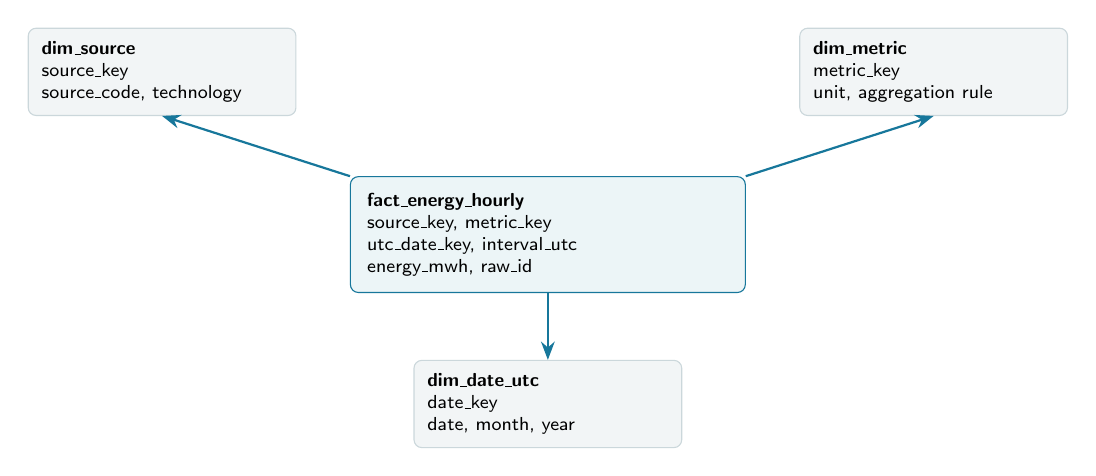
\begin{tikzpicture}[scale=.85,transform shape,>=Stealth,every node/.style={font=\sffamily\fontsize{8.1}{9.3}\selectfont},d/.style={draw=thinrule,rounded corners=1mm,fill=papergray,align=left,text width=36mm,inner sep=2mm},f/.style={draw=steelblue,rounded corners=1mm,fill=lightblue,align=left,text width=54mm,inner sep=2.5mm}]
\node[f] (f) {\textbf{fact\_energy\_hourly}\\source\_key, metric\_key\\utc\_date\_key, interval\_utc\\energy\_mwh, raw\_id};
\node[d,above left=9mm and 8mm of f] (s) {\textbf{dim\_source}\\source\_key\\source\_code, technology};
\node[d,above right=9mm and 8mm of f] (m) {\textbf{dim\_metric}\\metric\_key\\unit, aggregation rule};
\node[d,below=10mm of f] (t) {\textbf{dim\_date\_utc}\\date\_key\\date, month, year};
\draw[-{Stealth},steelblue,thick] (f.north west) -- (s.south);
\draw[-{Stealth},steelblue,thick] (f.north east) -- (m.south);
\draw[-{Stealth},steelblue,thick] (f.south) -- (t.north);
\end{tikzpicture}
\end{center}
\textit{Figure 4.2.} A minimal analytical star schema with clearly separated measures and descriptors; all nodes are author-created teaching designs.

\topic{4.6.3}{Energy/power units and additive measures}
MWh is additive across disjoint time intervals and distinct contributing sources \emph{when} the sources do not describe the same physical production twice. MW is a rate and usually needs a duration-weighted aggregation. A ratio such as renewable share is nonadditive: sum the component MWh values and \emph{then} divide, rather than averaging daily ratios without weighting. Every metric dictionary entry must state unit, time grain, population and admissible aggregation.
\repo{P039: Medallion and dimensional example}{https://github.com/Jb-Analytics/snowflake-dbt-tpch-medallion}


\textbf{Grain is a promise.} If the pipeline later accepts quarter-hour meter data, do not merely insert the new rows into this hourly fact. Either aggregate four complete disjoint intervals into one hour or introduce a separate quarter-hour fact with an explicit duration. A clear grain prevents a quiet semantic regression when a source changes its publishing frequency.

\newpage
% page 68
\section*{4.7\quad Keys, surrogate identifiers, and slowly changing dimensions}
\topic{4.7.1}{Natural versus surrogate keys}
A source code identifies an entity in the supplying system; a surrogate key identifies a row in our analytical dimension. The distinction matters when source systems change identifiers or when descriptive history must be retained. Keep both keys. Surrogate keys can be generated with sequences or identity mechanisms, but their numbers have no business meaning and should never appear as customer-facing descriptions.

\topic{4.7.2}{Slowly changing dimensions: types 1 and 2}
Type 1 overwrites a descriptive attribute when only the current correct description is needed. Type 2 preserves changes as separate effective-dated rows. If a generation facility changes its technology label, choose based on the reporting contract: should a 2024 report reproduce the label believed in 2024, or use today's corrected category? Neither answer is universally right. Type 2 requires an explicit validity range and a rule for late-arriving corrections.

\begin{lstlisting}[language=SQL,caption={Type 2 lookup: half-open validity interval.}]
SELECT f.raw_id, s.source_key
FROM book_ch04.fact_energy_hourly f
JOIN book_ch04.dim_source_history s
  ON f.source_code = s.source_code
 AND f.interval_start_utc >= s.valid_from_utc
 AND f.interval_start_utc < s.valid_to_utc;
-- A valid_to_utc sentinel or explicit NULL handling
-- must be declared in the dimension contract.
\end{lstlisting}

\topic{4.7.3}{Constraint enforcement caveats by table type}
In Snowflake standard tables, primary-key, unique and foreign-key declarations are typically \emph{informational}, not enforced. By contrast, \texttt{NOT NULL} and supported \texttt{CHECK} constraints are enforced; hybrid tables apply additional key-enforcement rules. Snowflake's current constraints documentation must be verified for the edition and table type used [7]. Tests for duplicate natural keys and missing dimension matches remain essential even if a model documents a primary key.

\begin{insight}\textbf{Don't mistake metadata for evidence.}\quad A declared primary key on a standard fact table is not proof that no duplicate rows exist. The release gate should count duplicate business keys over the actual data and fail if it finds any.\end{insight}
\repo{P042: Data Vault and dbt Snowflake modelling example}{https://github.com/ScalefreeCOM/datavault4dbt-snowflake-demo}


\textbf{History integrity.} For type-2 dimensions, reject overlapping effective intervals and document open-ended validity. Retroactive corrections may require replaying historical fact-to-dimension mappings.

\newpage
% page 69
\section*{4.8\quad Data validation and SQL testing patterns}
\topic{4.8.1}{Null, uniqueness, and range checks}
A useful data test states a falsifiable assertion with a known severity and an owner. In the energy platform, accepted observations must identify a source and metric, have a usable UTC interval start, hold a nonnegative interval energy value for the selected generation metric, and contain at most one accepted observation per source/metric/hour. A test that returns zero offending rows is easy to automate and review.

\begin{lstlisting}[language=SQL,caption={Failing rows: missing or negative accepted energy.}]
SELECT raw_id, source_code, interval_start_utc,
       energy_mwh
FROM book_ch04.fact_energy_hourly
WHERE source_code IS NULL
   OR interval_start_utc IS NULL
   OR energy_mwh IS NULL
   OR energy_mwh < 0;
\end{lstlisting}
\begin{lstlisting}[language=SQL,caption={Failing keys: more than one fact per grain.}]
SELECT source_code, metric_code,
       interval_start_utc, COUNT(*) AS n
FROM book_ch04.fact_energy_hourly
GROUP BY source_code, metric_code, interval_start_utc
HAVING COUNT(*) > 1;
\end{lstlisting}

Range rules need domain justification. Negative \emph{consumption} or net-flow metrics can be legitimate depending on the definition; a naive generic \texttt{value >= 0} test could erase meaningful sign conventions. Separate the rule for the \emph{generation\_mwh} metric used in this exercise from any generalized future metric that might have a different valid range. Likewise, a null \texttt{estimated\_flag} might mean ``unknown'' rather than ``no''.

\begin{whitebox}\textbf{Test specification.}\quad Each check must document its column scope, expected value or range, evidence of the business rule, result semantics (zero rows versus one summary row), severity, and remediation step.\end{whitebox}

\textbf{Expected fixture result.} After applying the declared correction rule to seven raw rows, the demonstration contains six accepted unique hourly observations. No accepted record has null or negative energy. These are \emph{expected results for the synthetic fixture}, not measurements from an actual Snowflake execution.
\repo{P043: Retail data engineering pipeline example}{https://github.com/Snowflake-Labs/sfguide-building-retail-analytics-de-pipeline}


\textbf{An operational metric.} A test that discovers 1 invalid row out of 7 has a different impact from one that discovers 1 invalid row out of 7 million. Preserve both absolute exception counts and normalized rates, and do not allow percentage dashboards to conceal a small number of serious defects. Define freshness and completeness checks as independent requirements: valid values from only one of two expected source systems still produce an incomplete national picture.

\newpage
% page 70
\topic{4.8.2}{Transformation reconciliation}
A model can pass uniqueness and null checks yet still lose a valid source during a join. Reconciliation compares what entered a controlled transformation with what emerged, at matched business grain. For our fixture, deduplication legitimately removes one superseded reading. Therefore \emph{raw row count = fact row count} is the wrong invariant. The correct checks are \emph{one accepted version per business observation}, complete coverage of expected observations, and preservation of totals calculated from those accepted versions.

\begin{lstlisting}[language=SQL,caption={Independent control total on accepted raw versions.}]
WITH ranked AS (
 SELECT source_code, metric_code, interval_text,
        TRY_TO_DECIMAL(mwh_text,18,3) AS mwh,
        ROW_NUMBER() OVER (
          PARTITION BY source_code, metric_code,
                       interval_text
          ORDER BY loaded_at_utc DESC, raw_id DESC
        ) AS rev_rank
 FROM book_ch04.raw_energy
), control AS (
 SELECT COUNT(*) AS n, SUM(mwh) AS mwh
 FROM ranked WHERE rev_rank = 1
)
SELECT * FROM control;
-- Synthetic fixture: expected n=6, mwh=97.500.
\end{lstlisting}

An independent target check should compare accepted source keys and row counts, then verify the energy sum. Use tolerances for approximate floating-point metrics; here exact scale-3 decimal totals are suitable. A failure should identify the source and hour, not merely report \texttt{FALSE}.

\begin{insight}\textbf{Failure mode: two wrongs reconcile.}\par
If the pipeline and its ``test'' both deduplicate with the same erroneous partition key, they can agree perfectly while both being wrong. A credible control calculation should use independent logic, fixture expectations, or a separately verified source contract.\end{insight}

Tests are operational agreements. A pipeline should stop publishing new gold data on a critical reconciliation failure, retain rejected rows and raw inputs for investigation, and avoid presenting partial totals as verified values. For a long-running platform, save the acceptance metrics with batch IDs and source snapshots for audit and replay.


\textbf{Reconciliation at scale.} Global totals are useful but insufficient when large positive and negative discrepancies cancel. Add per-source, per-metric and per-date reconciliation; include count and total, plus a list of missing or unexpected keys. Use stable batch identifiers to compare the same snapshot at each stage. Reconciliation must also consider whether a late revision is expected to restate a historical total or merely append a new publication event.

\newpage
% page 71
\topic{4.8.3}{SQL testing anti-patterns and corrections}
The most dangerous tests are those that look decisive but do not describe a business invariant. \texttt{COUNT(*) > 0} proves only that a table is nonempty. \texttt{DISTINCT} in the final query can hide a join fanout. \texttt{COALESCE(value,0)} converts missing measurements into numeric events. Choosing the latest row without deterministic ordering can produce different accepted values on otherwise similar runs. An assertion that joins two differently aggregated datasets can itself double-count and conceal a discrepancy.

\begin{center}
\small\begin{tabularx}{\linewidth}{@{}p{40mm}X@{}}\toprule
Fragile pattern & More defensible test\\\midrule
``Table has rows'' & Check expected source/date coverage and freshness.\\
``No \texttt{NULL} after \texttt{COALESCE}'' & Check raw parse failures before fallback is applied.\\
``\texttt{DISTINCT} fixed duplicates'' & Enforce and test business-key uniqueness upstream.\\
``Latest row wins'' & Specify revision authority and deterministic tie-breaking.\\
``Total matches yesterday'' & Reconcile to accepted source versions and batch IDs.\\
``Test passed once'' & Test every publication and track historical failures.\\\bottomrule
\end{tabularx}
\end{center}

A \emph{negative test} intentionally introduces a defect and verifies that the pipeline catches it. Insert a duplicate accepted business key in an isolated disposable copy; the uniqueness test must fail. Change one generated MWh value to a negative number; the domain check must identify it. Remove a required dimension row; the unmatched-fact check must detect a missing join. Never inject faults into shared or production tables, and always script cleanup.

\begin{lstlisting}[language=SQL,caption={Left anti-join: facts without matching source dimension.}]
SELECT f.source_code, COUNT(*) AS missing_matches
FROM book_ch04.fact_energy_hourly f
LEFT JOIN book_ch04.dim_source s
  ON f.source_code = s.source_code
WHERE s.source_code IS NULL
GROUP BY f.source_code;
\end{lstlisting}

\textbf{Release gate.} Define the failure categories \texttt{BLOCKER}, \texttt{WARNING}, and \texttt{INFORMATIONAL}; specify alert owner, replay strategy, and known accepted exceptions. The gate should be testable offline with synthetic fixtures even when cloud credentials are unavailable. The companion bundle includes such a validator rather than claiming a live Snowflake integration run.


\textbf{Avoid self-confirming tests.} When the transformation relies on a timezone conversion, a test that calls the exact same conversion on the same field can repeat its error. Write edge-case fixtures containing known UTC instants around both clock transitions and manually verified expected local labels. When a join uses effective dates, include a fixture on each boundary. Deliberately failing tests are often more informative than repeatedly passing the happy-path sample.

\newpage
% page 72
\section*{4.9\quad Naming, documentation, and maintainable SQL}
\topic{4.9.1}{Readable SQL and explanatory comments}
A SQL transformation is a maintained engineering artifact, not a one-time interactive answer. Maintainability starts with a predictable structure: name each CTE by its role, list only needed columns, place a join predicate beside the join, keep filters easy to audit, and expose grain-changing operations. A code review is easier when the business key appears consistently across staging, tests, and documentation.

\begin{lstlisting}[language=SQL,caption={A readability-oriented transformation sketch.}]
WITH accepted_readings AS (
    SELECT source_code, metric_code,
           interval_start_utc, energy_mwh
    FROM book_ch04.stg_energy_accepted
    WHERE metric_code = 'generation_mwh'
), matched_sources AS (
    SELECT r.*, s.source_key
    FROM accepted_readings r
    LEFT JOIN book_ch04.dim_source s
      ON r.source_code = s.source_code
)
SELECT source_key, interval_start_utc,
       energy_mwh
FROM matched_sources;
\end{lstlisting}

Do not use comments to restate the obvious (\texttt{-- select source key}). Explain assumptions that the SQL cannot express: why a late revision supersedes an earlier record, which physical sources may overlap, why a local date is used, and which source metadata authorizes a unit conversion. Comments should not disagree with the query; a stale comment is worse than none.

\begin{whitebox}\textbf{Naming convention for this book}\par
\texttt{raw\_*}: appendable source evidence; \texttt{stg\_*}: typed validated source-shaped data; \texttt{dim\_*}: descriptive context; \texttt{fact\_*}: measures at declared grain; \texttt{v\_*}: reader-facing views; \texttt{test\_*}: assertions returning violating rows. Names are descriptive, unquoted, and consistently snake\_case.\end{whitebox}

Avoid enforcing arbitrary style preferences as facts. Whether leading commas or trailing commas are used is much less consequential than a clear grain, a testable result and consistent formatting. Use SQL linting where feasible, but distinguish stylistic lint rules from semantic correctness checks.


\textbf{An editing criterion.} Prefer meaningful names over abbreviations that save a few characters but hide a contract. A future maintainer must know whether \texttt{energy\_mwh} represents final adjusted energy or raw preliminary energy. Make the column name and dictionary agree, then include one test that demonstrates the semantics. A SQL comment about a physical formula should identify its source and units so that it remains defensible if a provider modifies its measurement specification.

\newpage
% page 73
\topic{4.9.2}{Data dictionary and lineage}
A model is not documented until a new engineer can state what its measures mean without reading the entire transformation script. A \emph{data dictionary} records entity purpose, primary business grain, column types, descriptions, units, nullability expectations, acceptable value ranges, sources, and ownership. A \emph{lineage} record identifies the upstream inputs and transformations used to construct each important output.

\begin{center}
\small\begin{tabularx}{\linewidth}{@{}p{30mm}p{23mm}X@{}}\toprule
Column & Type & Meaning and rule\\\midrule
\texttt{source\_code} & VARCHAR & Source natural key; not null in accepted data.\\
{\fontsize{8.2}{9.7}\selectfont\texttt{interval\_start\_utc}} & {\fontsize{8.2}{9.7}\selectfont TIMESTAMP\_NTZ} & UTC hour start by contract; half-open interval.\\
\texttt{energy\_mwh} & NUMBER(18,3) & Accepted generation energy for one hour; additive when sources do not overlap.\\
\texttt{raw\_id} & NUMBER & Audit pointer to authoritative latest raw reading.\\
{\fontsize{8.2}{9.7}\selectfont\texttt{loaded\_at\_utc}} & {\fontsize{8.2}{9.7}\selectfont TIMESTAMP\_NTZ} & Source-record ingestion time, not measurement time.\\\bottomrule
\end{tabularx}
\end{center}

The distinction between \texttt{interval\_start\_utc} and \texttt{loaded\_at\_utc} is fundamental. A late source correction should change which raw record is accepted for a January measurement; it should not reclassify that measurement into October simply because the correction arrived then. Lineage must also preserve the revision-selection rule and make retained raw values inspectable.

\begin{center}
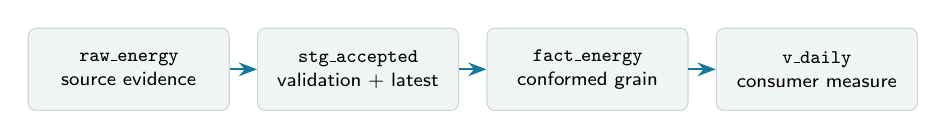
\begin{tikzpicture}[scale=.87,transform shape,>=Stealth,every node/.style={font=\sffamily\fontsize{8.3}{10}\selectfont},n/.style={draw=thinrule,fill=papergray,rounded corners=1mm,text width=27mm,minimum height=12mm,align=center}]
\node[n] (raw) {\texttt{raw\_energy}\\source evidence};
\node[n,right=4mm of raw] (stg) {\texttt{stg\_accepted}\\validation + latest};
\node[n,right=4mm of stg] (fact) {\texttt{fact\_energy}\\conformed grain};
\node[n,right=4mm of fact] (view) {\texttt{v\_daily}\\consumer measure};
\draw[->,steelblue,thick] (raw)--(stg);
\draw[->,steelblue,thick] (stg)--(fact);
\draw[->,steelblue,thick] (fact)--(view);
\end{tikzpicture}
\end{center}
\textit{Figure 4.3.} Model lineage identifies contracts between layers, not merely arrows between database objects.

For a production-ready project, store documentation beside versioned SQL and register the owner who can resolve disputes about meaning. The \texttt{data\_dictionary.md} file in the lab records assumptions and deliberately flags synthetic data so no example figures can be mistaken for Finnish national energy statistics.


\textbf{Field-level lineage.} For the fact table energy measure, trace the originating raw decimal text, the decimal parsing policy, the latest-revision ordering, the source and metric lookup, and the fact table's publication batch. For \texttt{interval\_start\_utc}, document the provider's UTC declaration and the parser used. These two traces allow a reviewer to answer: ``Which exact input established this amount, and which transformation made it reportable?''\par
\textbf{Change management.} Store the dictionary in version control together with SQL, tests and review decisions. If the source updates its unit from MWh to kWh, do not silently rename the same numeric column and continue. Record the new contract, add a unit conversion with explicit factor and validation, and backfill or distinguish historical partitions. The dictionary should specify the effective date of the change and the person who approved it.

\newpage
% page 74
\topic{4.9.3}{Naming policy and peer review}
A small team can produce a large operational risk by allowing multiple, incompatible definitions of ``daily generation.'' Agree on naming and semantic conventions before publishing dashboards. For example, \texttt{generation\_mwh\_utc\_day} is explicit about the interval basis; \texttt{total\_energy} may not be. The data contract should state whether the figure is gross or net generation, the role of imports and exports, the geographic coverage, and the day boundary.

A meaningful pull-request review tests five questions. \emph{Grain}: can two rows legitimately share the declared key? \emph{Units}: are the numbers additive or rates? \emph{Time}: which timezone, interval boundaries, and late-arrival rules apply? \emph{Correctness}: where are the independent controls and defect fixtures? \emph{Operations}: can the transformation be replayed safely and cheaply without broad privileges? These questions are more durable than review comments about capitalizing SQL keywords.

\begin{whitebox}\textbf{Review record: model version CH04-1}\par
Source shape: two synthetic generation sources, three UTC hours, one superseding revision. Accepted grain: one value per source, metric and UTC hour. Accepted observations: six. Expected generation: 97.500 MWh. Evidence: raw CSV checksum, offline validator output, SQL test queries, reviewer initials and Snowflake live-run date (blank until actually executed).\end{whitebox}

All example repositories in the external catalogue are \emph{research references}, not automatically licensed source files. The teaching implementation supplied with this chapter is original. Before importing external code, check its license and record the applicable commit. If a GitHub repository is missing, archived, or incompatible, the chapter should remain understandable and the companion lab should still run with its own disclosed test inputs.

\repo{P044: dbt Snowflake utilities}{https://github.com/Montreal-Analytics/dbt-snowflake-utils}
\repo{P045: dbt constraints examples}{https://github.com/Snowflake-Labs/dbt_constraints}

\textbf{End-of-model checklist.} A reader should be able to reconstruct a valid six-row fact, explain why an apparent seventh record is superseded, identify a faulty join before aggregation, and justify the timezone and units. Section 4.L provides the exact acceptance artifacts to verify these claims.


\textbf{Practical peer-review procedure.} Ask a second engineer to execute the offline fixture, inspect the accepted correction, and explain why it changes the aggregate by 0.500 MWh relative to the earlier record. Then ask that reviewer to delete a required dimension row from a disposable copy and demonstrate the orphan test failing. Record findings in a pull request rather than editing the expected result to make a failure disappear. Reviewers should also confirm that published SQL contains no credentials and that each destructive statement is scoped to an explicitly disposable schema.\par
\textbf{Edition control.} A published book inevitably outlives some vendor interfaces. Maintain an errata page and versioned companion code for API differences, but preserve the chapter's durable rationale: grain, units, joins, corrections and validation. Readers should be able to apply that reasoning even if a repository or user-interface menu changes.

\newpage
% page 75
\section*{4.L\quad Guided lab: a tested energy star model}
\topic{4.L.1}{Prerequisites, inputs, and cost guardrails}
\textbf{Inputs.} A synthetic CSV containing seven source events: six distinct source-hour observations and one corrected revision. The original reading for one solar hour is 12.500 MWh; its later authoritative version is 13.000 MWh. The accepted total is 97.500 MWh. These numbers are fictional and are not measurements of Finland's grid. Use only the dedicated \texttt{BOOK\_CH04} schema provisioned under Chapter 3's bounded laboratory account.

\textbf{Safe order:} (1) run the offline Python validator, (2) inspect its six accepted keys, (3) create a disposable transient raw table in the isolated schema, (4) execute staging and fact scripts, (5) run failure-returning tests and inspect row counts, (6) explicitly suspend the small warehouse and delete only approved disposable objects. A file labelled \texttt{cleanup.sql} is not permission to delete any table outside this lab.

\topic{4.L.2}{Procedure: parse, select revision, and materialize}
\begin{lstlisting}[language=SQL,caption={Illustrative model transformation; full script in bundle.}]
CREATE OR REPLACE TRANSIENT TABLE
 book_ch04.stg_energy_accepted AS
SELECT raw_id, source_code, metric_code,
       TRY_TO_TIMESTAMP_NTZ(interval_text)
          AS interval_start_utc,
       TRY_TO_DECIMAL(mwh_text,18,3)
          AS energy_mwh,
       loaded_at_utc
FROM book_ch04.raw_energy
WHERE TRY_TO_TIMESTAMP_NTZ(interval_text)
          IS NOT NULL
  AND TRY_TO_DECIMAL(mwh_text,18,3)
          IS NOT NULL
QUALIFY ROW_NUMBER() OVER (
 PARTITION BY source_code, metric_code,
              TRY_TO_TIMESTAMP_NTZ(interval_text)
 ORDER BY loaded_at_utc DESC, raw_id DESC
) = 1;
\end{lstlisting}

\textbf{Important.} The SQL above is a selected teaching excerpt. It intentionally uses a dedicated schema and an explicit parsing boundary, but production ingestion also needs format, rate, deduplication tie and source-identity contracts. Full bundle scripts add stable dimensions and an output fact. Nothing in these pages implies that a Snowflake account was connected or queried while this manuscript was prepared.

\begin{insight}\textbf{Required deliverables.}\quad \texttt{model.sql}; \texttt{sql-tests/}; \texttt{data\_dictionary.md}; \texttt{energy\_sample.csv}; \texttt{validate\_fixture.py}; and a README with account prerequisites, actual run evidence fields, troubleshooting, and cleanup controls.\end{insight}


\textbf{Why the fixture includes a correction.} A six-row flawless example would teach syntax but not the engineering reason for version selection. The seventh source event forces the reader to distinguish the raw audit log from the accepted observation table. Its known 0.500 MWh adjustment creates an independent numerical oracle for the test suite.

\newpage
% page 76
\topic{4.L.3}{Expected results, failures, rollback, and cleanup}
The seven-row synthetic fixture contains six accepted observations and 97.500 MWh after applying one solar correction. The offline validator checks these expectations independently. A live Snowflake run succeeds only when it matches these results and all blocker tests return zero violations. Record its edition, revision, query IDs and timestamp; do not present expected output as measured evidence.

\begin{lstlisting}[language=SQL,caption={Acceptance checkpoint for the isolated Snowflake lab.}]
SELECT COUNT(*) AS accepted_rows,
       SUM(energy_mwh) AS accepted_mwh
FROM book_ch04.fact_energy_hourly;
-- Expected on the synthetic fixture:
-- accepted_rows=6, accepted_mwh=97.500
\end{lstlisting}
\textbf{If results differ:} inspect rejected casts, timestamps, revisions, join fanout and filters before changing an expected value. Preserve raw input and logs. Restrict cleanup to named disposable objects and suspend the lab warehouse; otherwise costs may continue.

\topic{4.L.4}{Exercises and assessment rubric}
\begin{enumerate}
\item \textbf{Foundation.} Explain the difference among \texttt{NULL}, zero and a failed text-to-number conversion. Predict the result of a \texttt{LEFT JOIN} when the dimension row is missing.
\item \textbf{Practitioner.} Add a second source revision and design a test that fails if two accepted records share the same business key. Show the expected accepted-count change (or lack thereof).
\item \textbf{Architecture.} Decide whether daily national output belongs in a materialized view, normal view or persisted gold table. Defend your answer using read rate, update rate, feature limitations, costs and auditability.
\end{enumerate}
\textbf{Rubric (10 points).} Grain/units (3); deterministic revisions/time semantics (2); independent reconciliation/tests (3); safe operation/docs (2). \textbf{Pass:} at least 8/10 and no missing blocker.

\begin{whitebox}\textbf{Chapter 4 summary.}\quad Correct analytics needs grain, cardinality, time and unit semantics, safe conversions, and independent validation. Chapter 5 will ingest external files without losing this evidence.\end{whitebox}

\textbf{Documentation and further reading.}\par\vspace{-1mm}
{\fontsize{8.2}{10.2}\selectfont
[1] Snowflake, \href{https://docs.snowflake.com/en/sql-reference/data-types}{Data Types}.\quad [1] Snowflake, \href{https://docs.snowflake.com/en/user-guide/table-considerations}{Table Design}.\quad \par
[2] Snowflake, \href{https://docs.snowflake.com/en/sql-reference/functions/try_cast}{TRY\_CAST}.\quad [3] Snowflake, \href{https://docs.snowflake.com/en/sql-reference/functions-window-syntax}{Window Frames}.\quad \par
[4] Snowflake, \href{https://docs.snowflake.com/en/sql-reference/constructs/qualify}{QUALIFY}.\quad [5] Snowflake, \href{https://docs.snowflake.com/en/user-guide/tables-temp-transient}{Temporary / Transient Tables}.\quad \par
[6] Snowflake, \href{https://docs.snowflake.com/en/user-guide/views-materialized}{Materialized Views}.\quad [7] Snowflake, \href{https://docs.snowflake.com/en/sql-reference/constraints}{Constraints}.\quad \par
}

\end{document}
